\documentclass[12pt]{beamer}
\usepackage{amsmath,amssymb,caption,csquotes,float,tabularx}
\usepackage{minted}
\usepackage[utf8]{inputenc}
\usepackage[english]{babel}
\usepackage[backend=bibtex]{biblatex}
\addbibresource{lsr.bib}
\captionsetup[figure]{labelsep=period}
% \captionsetup[table]{labelsep=period}
\definecolor{bg}{rgb}{0.95,0.95,0.95}
\hypersetup{
    colorlinks=true,
    linkcolor=blue,
    filecolor=blue,      
    urlcolor=blue,
    citecolor=cyan,
}
\usemintedstyle{emacs}
\usetheme{Madrid}
\begin{document}
\title{Hardware/Algorithm Co-design of Natural Language Processing Tasks}
\subtitle{Literature Search \& Review Presentation}
\author{Yihua Liu}
\institute{UM-SJTU Joint Institute}
\date{\today}
\begin{frame}
    \titlepage
\end{frame}
\section{Motivation}
\begin{frame}{Motivation}{Why Hardware Acceleration for Neural Networks?}
    \begin{itemize}
        \item Neural network are getting increasingly popular for a wide range of applications
        \item More embedded devices are deployed for neural network computation due to limitations of data transfer
        \item Resources are wasted when computation is done by traditional architecture
    \end{itemize}
    \begin{block}{Challenges}
    \begin{itemize}
        \item Computation resources of embedded devices are strictly limited
        \item Computation load of neural network are getting heavier because of larger datasets and more complex structure
        \item Improve energy efficiency while accuracy not decreased
        \item Need to be flexible for different applications and scalable for different computation load
    \end{itemize}
    \end{block}
\end{frame}
\section{Novelty}
\begin{frame}{Novelty}
    \begin{center}
        The first complete general hardware/algorithm co-design for state-of-the-art natural language processing tasks
    \end{center}
    \begin{itemize}
        \item Specialized datapath support for early-exit assessment, softmax and attention span masking, and layer normalization
        \item Non-volatile and high density storage of the shared multi-task parameters
        \item On-demand dynamic voltage/frequency scaling aided by integration of fast-locking all-digital phase-locked loop and low-dropout regulator
        \item Compressed sparse matrix execution via bitmask encoding \cite{tambe2021edgebert}
    \end{itemize}
\end{frame}
\section{Main Approach}
\begin{frame}{Main Approach}
\begin{figure}[H]
    \centering
    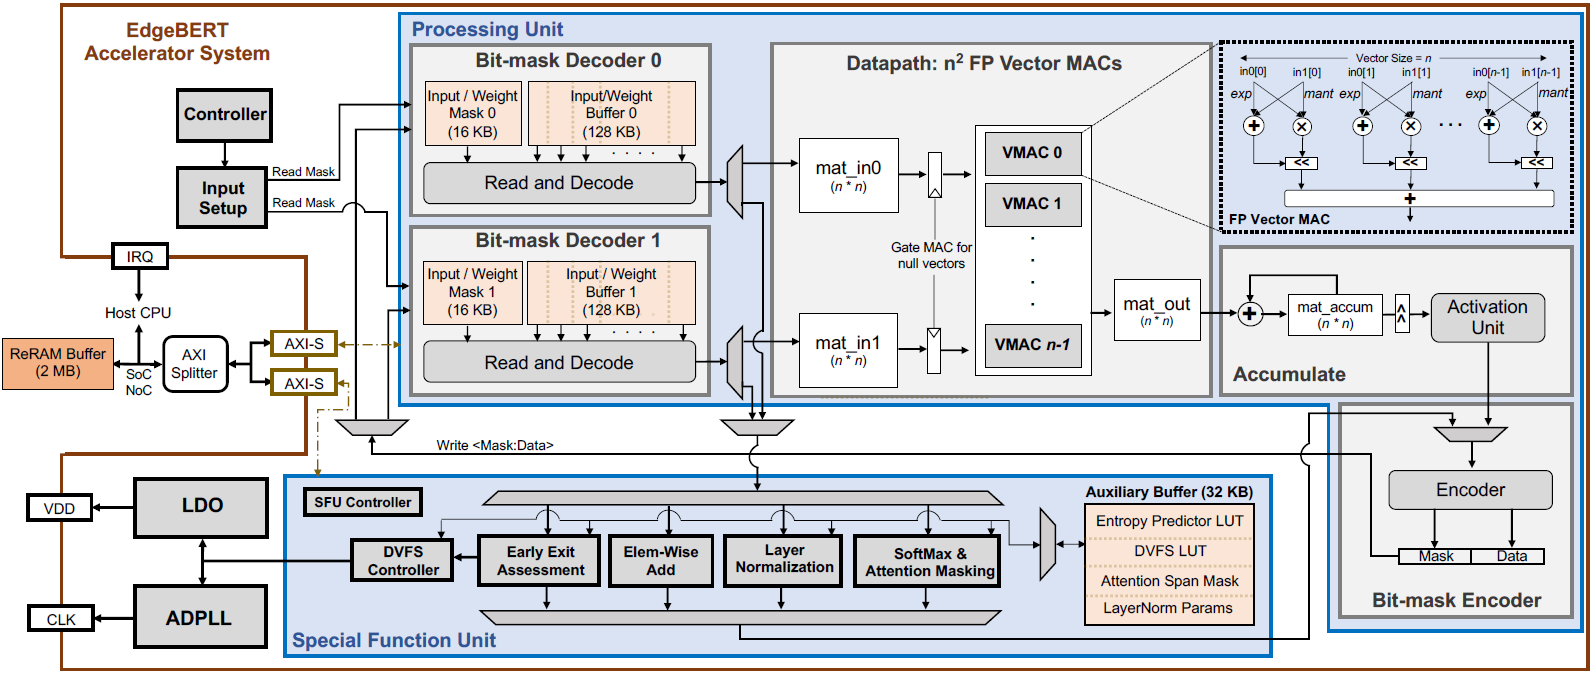
\includegraphics[width=1\textwidth]{1.png}
\end{figure}
\end{frame}
\section{Evaluation}
\begin{frame}{Evaluation}
    \begin{figure}[H]
        \centering
        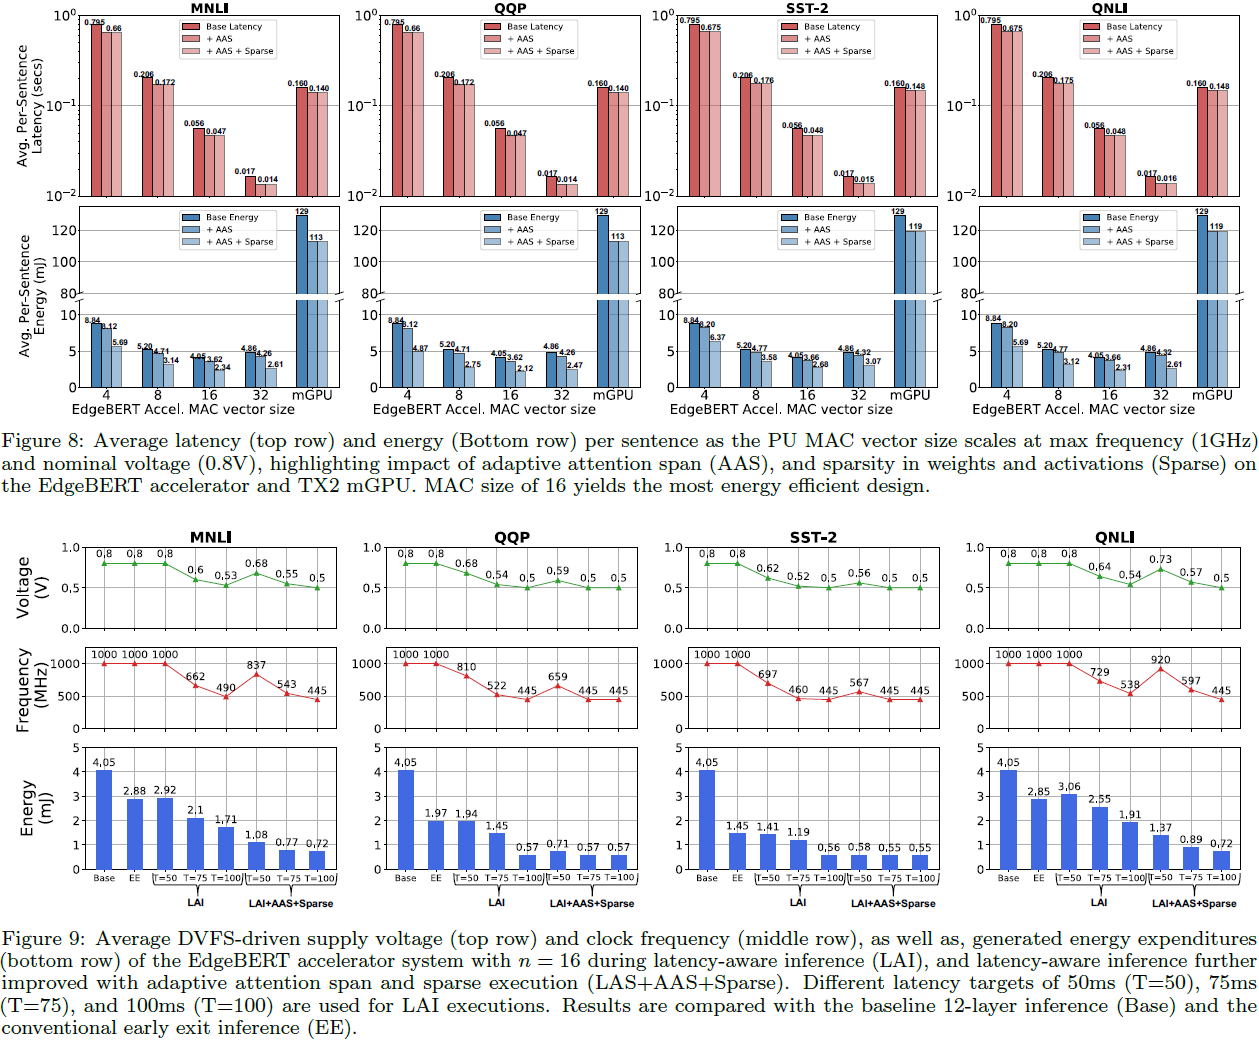
\includegraphics[width=0.8\textwidth]{2.png}
    \end{figure}
\end{frame}
\begin{frame}{Evaluation}
    \begin{figure}[H]
        \centering
        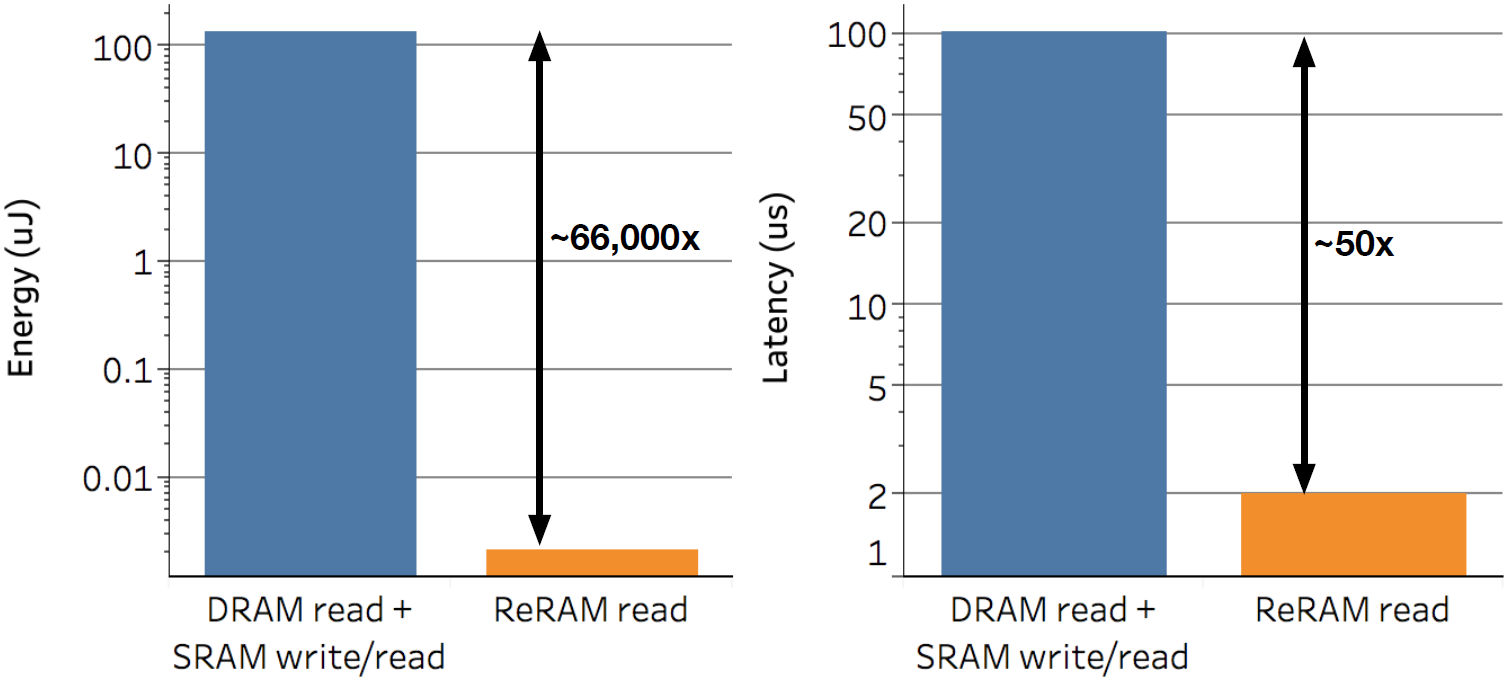
\includegraphics[width=0.8\textwidth]{3.png}
    \end{figure}
    \begin{itemize}
        \item Energy savings (per-inference): 7$\times$ compared to conventional inference and 2.5$\times$ compared to early-exit inference.
        \item Latency advantage 50 $\times$ greater than conventional operation and energy advantage 66,000 $\times$ greater than conventional operation.
    \end{itemize}
\end{frame}
\section{Limitations}
\begin{frame}{Limitations}
    \begin{itemize}
        \item Only support GLUE (General Language Understanding Evaluation) benchmark, not supporting Hugging Face datasets or SQuAD (Stanford Question Answering Dataset).
        \item Only test on Nvidia Jetson Tegra X2 board, not tested on latest Jetson Xavier NX board.
        \item It once claimed in previous versions that its solution leads to only 1\%-pt drop in accuracy \cite{tambe2021edgebert}, but it lacked data support, and it is removed from the latest version, so its accuracy drop is questionable.
        \item It admits that its eNVM modeling methodology is traditional ReRAM (Resistive RAM) arrays rather than emerging NVM technologies like PCM (Phase-Change Memory).
    \end{itemize}
\end{frame}
\section{Reference}
\begin{frame}{Reference}
    \printbibliography
\end{frame}
\section{Thanks}
\begin{frame}
\begin{center}
    \Huge Thanks!
\end{center}
\end{frame}
\end{document}
